\newchapter{intro}{Introduction}

This is the introductory text.

%\newsection{partPhys}{Particle Physics}

%\newsection{accelIntro}{Particle Colliders}

\newsection{linColliderIntro}{Motivation for Future Linear Colliders}

\newsection{clicIntro}{CLIC}

%\newsection{fontIntro}{FONT}

\newsection{clicPFF}{Phase Feedforward for CLIC}

\newsection{ctfIntro}{CTF3}

\subsection{Goals of CTF3}
\label{ss:ctfGoals}

CLIC and PFF

\subsection{Layout of CTF3}
\label{ss:ctfLayout}

\begin{figure}
  \centering
  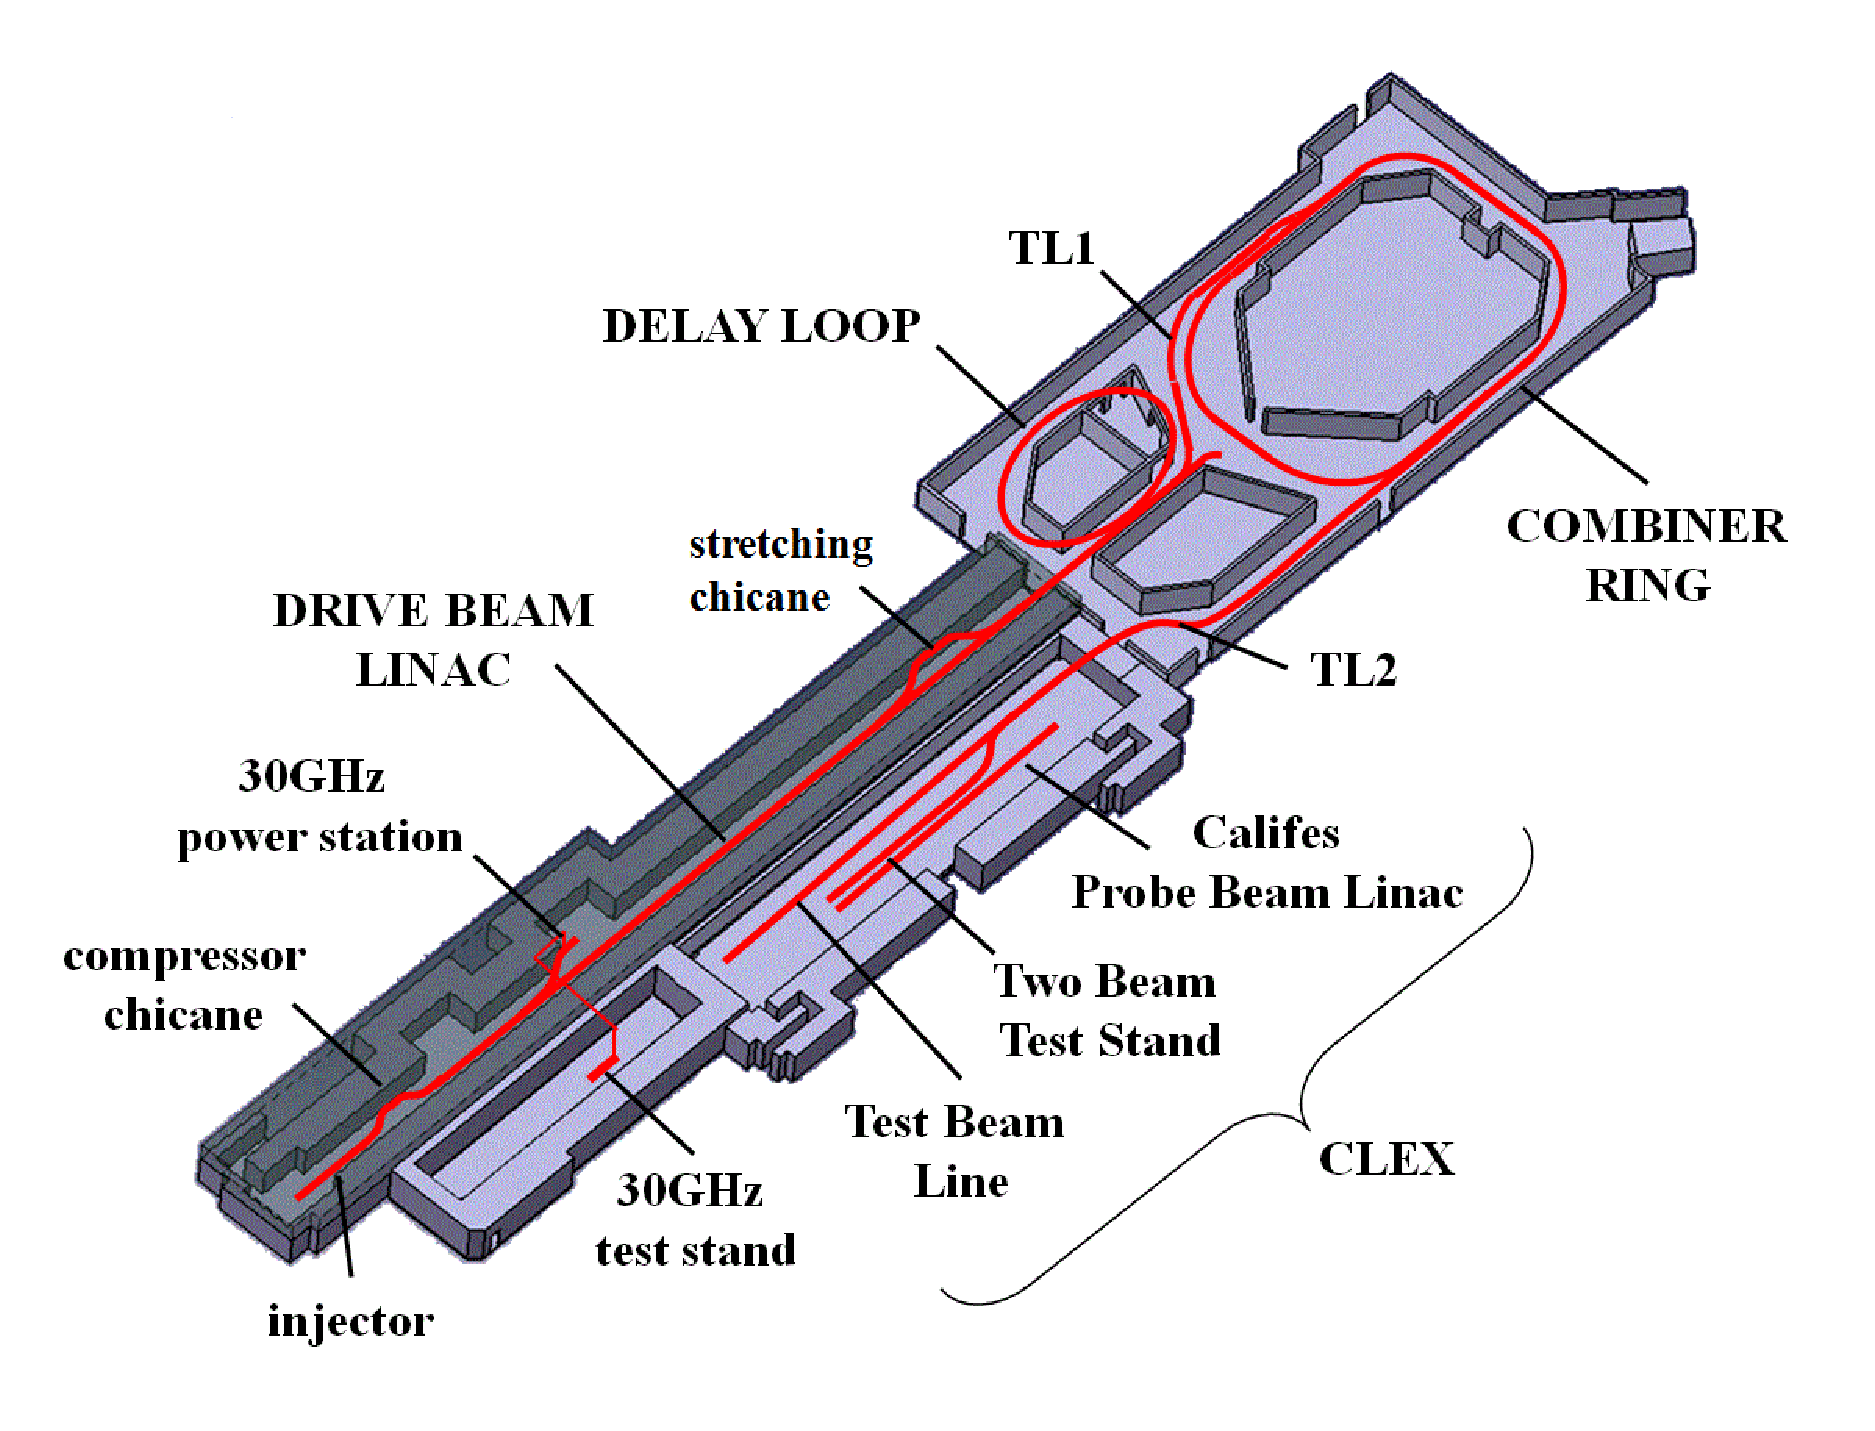
\includegraphics[width=0.45\textwidth]{Figures/ctfLayout}
  \caption{CTF3 schematic.}
  \label{f:ctfLayout}
\end{figure}

\newsection{pffCTFIntro}{Design of the PFF Prototype at CTF3}

\subsection{Schematic Overview of PFF System}
\label{ss:ctfPFFLayout};

\subsection{Hardware}
\label{ss:ctfPFFHardware}

\subsection{Latency}
\label{ss:availLatency};

\newsection{ctfVsCLIC}{Differences Between PFF at CTF and CLIC}

\subsection{Phase Sag}
\label{ss:phaseSag}

\subsection{Pulse Length}
\label{ss:pulseLength}

\newsection{phaseJitDefs}{Definitions of Different Phase Statistics}

Definitions of different types of phase jitter.


mean phase

phase along pulse

flatness?

zero phase?


\newsection{thesisOverview}{Thesis Overview}





